\documentclass[10pt]{article}
\usepackage[margin=.72in]{geometry}
\usepackage{amsmath,amssymb,graphicx,booktabs,hyperref}
\hypersetup{colorlinks=true,urlcolor=blue}
\setlength{\parindent}{0pt}
\setlength{\parskip}{6pt}
\newcommand{\LL}{\mathcal L}
\newcommand{\ord}{\operatorname{ord}}
\begin{document}
{\LARGE\bf Joint-six discovery}\par
{\large Interpolation obstruction and a product-jet target}\par
24 November 2026 \hfill Written analysis; producer unsigned/unverified

\textbf{Scope.} A complete written argument rejects one interpolation
certificate family at every multiplicity. A separate classical product
formulation specifies a joint-six selection target. No scientific/native
call, Lean endpoint, timing or solver run is added.

\textbf{The two existing regular charts.}
In characteristic different from2, for finite $R=(r_0,s_0)$ with
$s_0\ne0$ on the nonsingular Montgomery curve,
put $H=5O+R$ and $\phi_R=(y+s_0)/(x-r_0)$. The section basis is
$1,x,y,x^2,xy,\phi_R$. Normalizing $xy$ leaves $D=4O+R$, received
function $\rho=-xy$; normalizing $\phi_R$ leaves $D=5O$,
$\rho=-\phi_R$. Both have $D=H-T$ of degree5 and
$\rho\in\LL(H)\setminus\LL(D)$, with $T=O$ or $R$.

\textbf{Written theorem (exact hypotheses).}
Let $N\ge8$ distinct rational points avoid $\operatorname{supp}(H)$,
$T$ and $\operatorname{supp}(A)$, where $A$ is any divisor. For $s\ge1$,
let
\[
 Q(Z)=\sum_i a_i Z^i,\qquad a_i\in\LL(A-iD),\qquad d=\deg A,
\]
have total local multiplicity at least $s$ at each
$(P_j,\rho(P_j))$ on $E\times\mathbb A^1$. Then
\[
 \boxed{d<6s\ \Longrightarrow\ Q=0,\qquad
 d=6s\ \Longrightarrow\ Q=b(P)(Z-\rho)^s.}
\]
In the second assertion $Q\ne0$ and $b\ne0$ is a rational function;
its coefficient condition is $\operatorname{div}(b)+A-sH=0$.
For $A=sH$ the universal polynomial $(Z-\rho)^s$ exists. Its only
function-field root is $\rho$, outside the message space. The threshold8
is sufficient; optimality in the number of points is not asserted.

\textbf{Proof.}
For nonzero $F=\sum f_iZ^i$ define
$W_D(F)_v=\max_i(iD_v-v(f_i))$. A weighted Gauss valuation gives
$W_D(FG)=W_D(F)+W_D(G)$. To check cancellation, take the largest index
attaining minimum weighted valuation in each factor; their product is
the unique minimum term at the sum of those indices. Hence
$W_D(Z-\rho)=H$ and division by this factor decreases the budget by $H$.
After $t$ divisions, write $u=s-t$, $B=A-tH$, $e=d-6t$ and
$l=\deg_Z F$. The nonzero leading coefficient lies in $\LL(B-lD)$,
so $5l\le e$. Substitution gives $F(\rho)\in\LL(B+lT)$.
If this function were nonzero, its $Nu$ zeros would imply
\[
 Nu\le e+l\le \tfrac65 e\le \tfrac{36}{5}u<8u\le Nu,
\]
a contradiction. Thus $Z-\rho$ divides $F$. At each interpolation point
this graph factor has local order1; orders add in the regular local
ring, so the quotient has multiplicity at least $u-1$.
Repeat $s$ times. The final budget is negative when $d<6s$;
when $d=6s$, the leading-coefficient bound forces degree0 in $Z$.
This proves both conclusions. DERIVATION.md gives all divisor/local steps.

\textbf{Route decision.}
The standard six-agreement GS degree certificate is unavailable in these
charts. Raising multiplicity/list degree does not change the argument.
Frobenius-sparse powers with total multiplicity $p^e s$ also fit it.
Other decoders, nonuniform multiplicities, exceptional charts and joint
coefficient solving require separate analysis. A capped/incomplete solve
remains inconclusive. This is written algebra, not independent verification.

\newpage
{\Large\bf A different joint-six condition}\par
\textbf{A finite physical-base product.}
For a finite \emph{set} $X$ of distinct regular raw curve points, excluding
$O,\pm R$ and the original exceptional strata, put
\[
 f_c(P)=xy+c_0+c_1x+c_2y+c_3x^2+c_5\phi_R,\qquad
 F_R(c)=\prod_{P\in X} f_c(P).
\]
Each factor is affine linear in five coefficients with $c_0$ coefficient1.
At $c^*$ its vanishing factors have order1 and the others are units;
lowest homogeneous parts multiply in a polynomial domain. Therefore
\[
 \operatorname{mult}_{c^*}(F_R)
 =\#\{P\in X:f_{c^*}(P)=0\}\le6.
\]
The inequality uses the nonzero section's pole bound $H$. Consequently
six distinct section zeros are equivalent to
\[
 D^{[\alpha]}F_R(c^*)=0\quad(|\alpha|<6),\qquad
 \#\{\alpha\in\mathbb N^5:|\alpha|<6\}=\binom{10}{5}=252.
\]
Their divisor exhausts $H$, giving raw sum $R$ by the elliptic divisor
law in this distinct regular stratum. Original branch, index and
$[8]$-image replay are still required.

\textbf{Circuit implication and its limit.}
An \emph{exact} product circuit of length $L$ can be evaluated in
$k[\epsilon_0,\ldots,\epsilon_4]/(\epsilon)^6$, an algebra of dimension252.
Its output contains all252 Hasse jets. Naive truncated multiplication
gives $O(252^2 L)$ scalar work. Division requires a nonzero constant
term and an explicit unit guard. This preserves an \emph{evaluation}
exponent; it gives no coefficient selection or rootfinding bound.
The product degree is still $|X|$, with derivative degrees growing
accordingly. Repeated physical points repeat factors and can manufacture
sixfold multiplicity from one simple curve zero.

\begin{center}
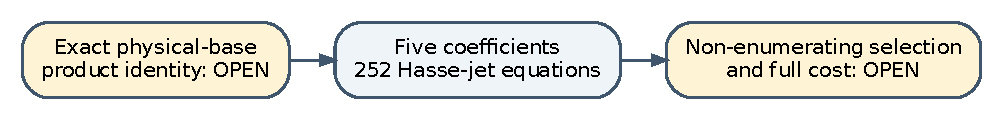
\includegraphics[width=\linewidth,height=.75in,keepaspectratio]{flow.pdf}
\end{center}

\textbf{Ordered next work.}
First prove that a norm/resultant of the frozen quotient-query
recurrence represents this exact physical-base product, up to declared
nonzero factors. Rationality, aliases, branches and nonunit strata
are part of that identity. It is proposed, not established here.
Then develop a separately versioned Rust jet compiler and a
non-enumerating coefficient-selection/root algorithm. A candidate-section
evaluation API must remain distinct from discovery. Do not scale a
generic solve from the fixed equation count or enumerate triples.

\textbf{Exponent-facing acceptance.}
The earlier conditional model's $\gamma<3$ optimized-family target
($\gamma<2$ at fixed $B\sim\ell^{1/6}$) is unchanged. Charge complete
setup, failed selection, memory, indexing, original witnesses, useful
target yield, rank/private tags/kernel and scalar recovery. No new
scientific job or campaign is scheduled.

\textbf{Primary sources and standing.}
Beelen--Montanucci (2025), Definition3 and
Theorems4--5 (local multiplicity, GS coefficient spaces and inseparable
variant); Snowden's Math679 Lecture2 (divisors and genus1 spaces);
Kopparty--Saraf--Yekhanin2011, Definitions5--6 (Hasse multiplicity);
Wakefield--Yoshinaga2007, Sections1--2 (arrangement derivative ideals).
SOURCES\_CHECKED.md records direct links and the separate power-decoder
scope. These are classical ingredients. KB unavailable; no novelty
clearance, independent signed theorem or performance claim.
\end{document}
